\documentclass{report}
\usepackage{titlesec}
\usepackage{color}   %May be necessary if you want to color links
\usepackage{pdfpages}
\usepackage{hyperref}
\usepackage{graphicx}

\hypersetup{
    colorlinks=true, %set true if you want colored links
    linktoc=all,        %set to all if you want both sections and subsections linked
    linkcolor=blue,  %choose some color if you want links to stand out
}

\titleformat{\chapter}{\normalfont\huge}{\thechapter.}{20pt}{\huge}

\begin{document}

\title{Notes: The Term Structure of Inflation Expectations}
\maketitle
 
\tableofcontents{}
 
\chapter{Old version}
In this section I will highlight some of the errors that I found in the August 2010 revision of Adrian and Wu (2009). Fixing these errors and re-estimating the model produces results that are qualitatively \textit{roughly} similar, but quantitatively different from the original results.\\

\section{Errors}

\begin{itemize}

\item The \textit{10-year expected inflation} series plotted in Fig 5 of Adrian and Wu (2009) only takes into account the first inflation factor. This could possibly be a remnant from the previous version of this paper, in which there was only one factor for inflation. When this is fixed and the second factor is also included, the gap between the `breakeven 10-year' and `expected inflation 10-year' series in Fig. 5 increases a little. Consequently, we see a shift up in the risk premia and the pre-crisis lows are 0.5\% rather than 0\%. This can be seen in pg.5 of \texttt{Figs-Orig-Reest-Parms.pdf}

\item After solving equations 14 and 15 to get $C_0$ and $C_1$, the final coefficients for the 3-month T-bills are not divided by the time to maturity, $\tau$.

(Since the 3-month T-bills data is also being used to estimate the model, I have included this information in the .tex file of the paper. This was not mentioned in the earlier version of the paper.)

\item An older version of the GARCH toolbox was producing erroneous estimates for the initial weeks, which was causing problems in the log-likelihood estimation. This has been fixed.

\item $\hat{\epsilon}^y_{t+1}$ are the residual of a regression of nominal yields on lagged nominal and real yields, and $\hat{\epsilon}^r_{t+1}$ are the residuals of a regression of real yields on lagged real and nominal yield. However, in the original code, $\hat{\epsilon}^y_{t+1}$ is being defined as the residual of a regression of nominal yields on just the lagged nominal yields, and $\hat{\epsilon}^r_{t+1}$ is being defined as the residual of a regression of real yields on just the lagged real yields. This has been fixed.


\end{itemize}

 
\section{Fixed output}
 
After fixing the aforementioned errors and re-estimating the model with some minor improvement to the estimation strategy, we find that although the qualitative results do not change, quantitatively, there is an approximately 50bp rise in the 10-yr risk premium prior to the crisis. This can be seen in the figure below, which plots the results from re-estimating the model on date from 2003-2009.
\begin{center}
\includegraphics[page=5, trim={5cm 6cm 5cm 6.5cm}]{Figs-Orig-Reest-Parms.pdf}
\end{center}

One thing to note, however, is that the 10-year inflation expectation generated by the model still falls to -1.5\% around 2009. This is in contrast to the survey measures of long-term inflation during that period.\\

\texttt{Figs-Orig-Reest-Parms.pdf} contains all the figures from Adrian and Wu (2009) constructed using the re-estimated model.


\chapter{Re-estimating the modified model on a larger dataset}
In this section I re-estimated the model on a larger dataset spanning 2003--2016. This significantly changes the results. In particular, the inflation risk premium, which was originally estimated to rise between 2008 and 2010, now falls during the same period. At the end of this section I will mention some possible ways to fix/improve these results.

\section{Output}
There are three major results that stand out from estimating the model on the larger dataset:
\begin{itemize}
\item There is a significant level shift up of the risk premium;
\item The risk premium actually falls around 2009, which is the opposite of the results from estimating the model on data from 2003--2009.
\item The expected inflation stays negative throughout the estimation period.
\end{itemize}

These results are displayed in the figure below (and the complete set of graphs are contained in \texttt{Figs-Orig-Reest-Parms-alldata.pdf}):

\begin{center}
\includegraphics[page=5, trim={5cm 6cm 5cm 6.5cm}]{Figs-Reest-Parms-alldata.pdf}
\end{center}

 
\section{Suggestions for improvement}
 
One of the starkest implications of estimating the model on a larger dataset is that the inclusion of post-2010 data results in the inflation risk premium to drop, instead of surge, between 2008 and 2010. The post-2010 slump in real rates, in which they even turned negative, could possibly be one reason for the model's results changing. We could fix this by imposing parameters restrictions. Preliminary tests show that this could be a promising direction.\\

I have already made some improvements to the code, which allow for a faster estimation of the model. I have also parallelized the code to take advantage of a 24-core high performance computer that I have access to in the Johns Hopkins Economics Department. This should make running counterfactuals and estimating the model significantly faster.\\

Files \texttt{fixing\_each\_parms\_to\_old.pdf} and \texttt{fixing\_each\_parmsind\_to\_old.pdf} contain results from imposing various parameter restrictions. (Explanation in separate file.)

\end{document}